%==============================================================================
% method.tex — Methodology for PP-HFM
% Self-contained \section{}; \input this into main.tex (never compile alone).
%
% Structured after the house methodology template: domain motivation, then a
% blueprint subsection, then one subsection per component (motivation ->
% description -> placement -> transition), with every equation gathered into a
% final formulation subsection.
%
% Required in the host preamble:
%   amsmath, amssymb, booktabs, algorithm, algorithmic, graphicx
% READABILITY PASS 2026-10-21: formal register; inter-subsection transitions
% removed; misplaced group-privacy sentence restored to its paragraph; the
% wrong forward reference before the deployment subsection fixed. Floats and
% equations are copied verbatim.
%==============================================================================

\section{Methodology}
\label{sec:method}

\subsection{Problem Statement}
\label{sec:method:problem}

Multimodal Internet-of-Things deployments combine sensing streams of different
kinds, such as physiological monitors with clinical records or inertial sensors
with video, at the location where the streams are produced. The training data
are therefore distributed, and in clinical settings they cannot be centralized,
because consent and data-protection regulations prohibit pooling. Federated
learning addresses this by moving the model instead of the data, but it does
not provide a privacy guarantee, because client updates are functions of the
client's records. A suitable framework must therefore combine distributed
multimodal training with a formal guarantee, within the network, latency and
energy constraints of an edge installation.

Differentially private federated learning provides such a guarantee, but the
\emph{unit} of the guarantee in clinical settings has received little
attention. Standard differentially private stochastic gradient descent
\cite{ref6} clips and accounts per training record. In a monitoring dataset, a
record is a fixed-length window rather than a person, and every patient in the
cohort used here contributes several windows. A record-level budget therefore
bounds whether a particular window was used in training, whereas a clinical
guarantee must bound whether a particular \emph{patient} was. Prior federated
systems address only one side of this problem. HED-FL \cite{ref3} provides a
hierarchical tier without differential privacy, FL2DP \cite{ref9} provides
differential privacy without a hierarchy, and neither these nor the
heterogeneity-aware and assignment-oriented designs \cite{ref4, ref5} model
multiple modalities per record or the grouping of records by individual.

The problem addressed is therefore the following. Several institutions each
hold multimodal recordings of their own patients, every patient contributes
many records, and no record may leave its institution. A shared model must be
trained through a client--edge--cloud hierarchy such that
\begin{enumerate}
\item the participation of any single patient, with all of their records, is
protected by a formal $(\varepsilon,\delta)$ guarantee that covers every
message the system releases, edge tier included;
\item the model remains close in utility to an identical non-private system;
and
\item the system remains deployable on IoT infrastructure, with low uplink
traffic, reliable delivery, low inference latency and low energy.
\end{enumerate}
These requirements interact. Protecting patients instead of records reduces
the number of protected units and therefore raises the relative noise;
clients partitioned by institution differ greatly in size, so a noise level
fitted to the smallest client degrades every larger one; and an edge tier
changes how many optimization steps each client takes, and hence how much of
its budget it spends. Table~\ref{tab:objectives} turns the three requirements
into seven quantitative targets, fixed before any experiment was run.

\subsection{Overall Framework of the Proposed PP-HFM}
\label{sec:method:overview}

This work therefore proposes a framework in which the privacy unit is the
patient by construction, and in which the hierarchy and the guarantee are
designed jointly. The system, PP-HFM (Patient-Private Hierarchical Federated
Multimodal learning), has three tiers: institutional clients that hold
patient-grouped multimodal records and never release them, edge aggregators
that perform several local rounds before communicating upward, and a cloud
aggregator that maintains the global model. Within each client, representation
learning is separated from private adaptation. Encoders pretrained on a
disjoint public population are frozen, and only a compact fusion head is
trained under a differentially private objective with patient-level
sensitivity. Fig.~\ref{fig:pphfm_arch} shows the overall organization.

\begin{figure*}[!t]
\centering
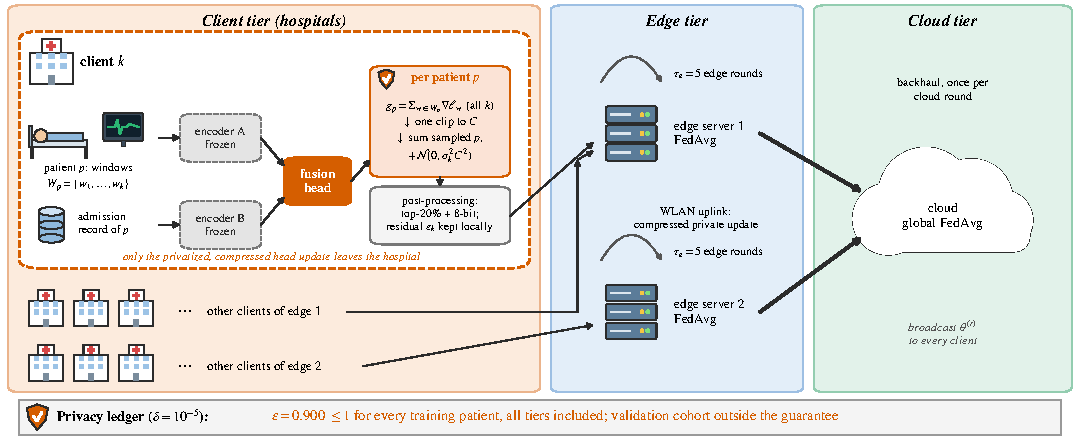
\includegraphics[width=\textwidth]{fig01_overview_core.pdf}
\caption{Architecture of PP-HFM. Each institutional client holds
patient-grouped multimodal records that never leave the institution, runs
frozen pretrained encoders, and privately trains only the fusion head, with
gradients summed per patient before clipping. Two edge aggregators perform
$\tau_e$ rounds of weighted averaging for every cloud round, and the cloud
averages the noisy, compressed updates globally.}
\label{fig:pphfm_arch}
\end{figure*}

Each client samples a batch of patients rather than windows, sums the
gradients of all windows of each sampled patient into one per-patient
gradient, clips that gradient, and adds noise to the aggregate once per
optimization step. The influence of any individual on the released model is
therefore bounded regardless of the number of records contributed. The
resulting update is compressed and sent to the client's edge, which averages
the updates of its clients. After several edge rounds, the edges report to the
cloud, which averages across edges and redistributes the global model.

The framework comprises the following components, each described in one of
the following subsections.
\begin{enumerate}
\item \emph{Frozen multimodal backbone} (Section~\ref{sec:method:backbone}):
fixed encoders, one per modality, and a compact trainable fusion head.
\item \emph{Patient-level privacy mechanism}
(Section~\ref{sec:method:privacy}): enforces sensitivity with respect to the
individual.
\item \emph{Noise calibration across clients}
(Section~\ref{sec:method:calib}): meets the budget for every client despite
large differences in client size.
\item \emph{Two-tier aggregation} (Section~\ref{sec:method:agg}): produces
the global model while using the wide-area link once per several local rounds.
\item \emph{Update encoding} (Section~\ref{sec:method:encoding}): reduces the
transmitted payload.
\item \emph{Deployment path} (Section~\ref{sec:method:deploy}): executes the
released model within a latency budget.
\item \emph{Network and energy instrumentation}
(Section~\ref{sec:method:instr}): measures the communication and energy costs
of the hierarchy.
\item \emph{Empirical audit} (Section~\ref{sec:method:mia}): tests the
resulting guarantee by membership inference.
\end{enumerate}
The encoder architecture and the aggregation rule
are adopted from established work and are not claimed
as contributions.

\subsection{Overall System Architecture}
\label{sec:method:arch}

PP-HFM is a three-tier federated system built on a frozen multimodal backbone.
Responsibilities are separated: the encoders provide fixed representations, a
compact head contains all trainable and privatized parameters, an edge tier
absorbs local rounds to reduce wide-area traffic, and a cloud tier maintains
the global model. The encoder design and the weighted averaging rule are
adopted from prior work. The design
contribution lies in the unit at which privacy is enforced and in the
accounting of the reported budget.

The architecture is shown in Fig.~\ref{fig:pphfm_arch}. An institutional
client holds a set of patients, each contributing several time-aligned
multimodal records. The records are encoded by two frozen modality-specific
encoders and combined by a trainable fusion head. The head is optimized under
a differentially private objective, and its compressed update is the only
quantity that leaves the institution. Updates are averaged at the edge over the
clients it serves. After $\tau_e$ such rounds, the edge models are averaged at
the cloud and redistributed. No record, single-record gradient or uncompressed
update crosses an institutional boundary.

The system consists of three functional groups. The first is the frozen
backbone: two modality-specific encoders, pretrained on a population disjoint
from every federated client and not adapted during federated training. The
second is the privatized trainable component: the fusion head, the
patient-level clipping and noise mechanism that governs its optimization, and
the calibration procedure that sets the noise scale. The third comprises the
communication components: the update encoding and the two-tier averaging.

Information flows in a group-then-bound structure. Within a client, records
are encoded and combined by the head, and gradients are grouped \emph{by
patient} before clipping, so that the clipped quantity is a patient's total
contribution rather than a single record's. Noise is added once to the
aggregate of the clipped per-patient gradients, after which the update is
compressed and transmitted. Communication is hierarchical: client to edge in
every edge round and edge to cloud once per cloud round, with the ratio set by
$\tau_e$.

This design follows from the constraints of the setting. Grouping gradients by
patient before clipping makes the guarantee a statement about individuals, and
avoids the severe degradation of a group-privacy conversion. Restricting
private optimization to a small head over frozen features keeps the dimension
of the perturbed vector low, which is necessary for acceptable utility under a
tight budget. Pretraining the features on a disjoint population keeps the
guarantee valid end to end. The edge tier reduces wide-area transmissions by a
factor of $\tau_e$ without changing the learning objective. Because the
encoders are fixed and the aggregation rule is standard, observed differences
can be attributed to the privacy unit and its accounting rather than to the
representation or the averaging.

\subsection{Frozen Multimodal Backbone}
\label{sec:method:backbone}

A tight privacy budget requires a large noise scale, and the noise a parameter
vector must absorb grows with its dimension, so private training of a full
network degrades severely. Parameter-efficient differentially private
fine-tuning, which restricts private optimization to a small trainable subset
over frozen pretrained features, is considerably more robust at small
$\varepsilon$ than end-to-end private training \cite{ref12, ref13}. PP-HFM
adopts this design unchanged. The framework adds the condition under which the
resulting guarantee remains valid, and a measurement of the cost of that
condition.

The backbone consists of two modality-specific encoders. The temporal encoder
takes a multichannel physiological time series as input. A multi-scale
convolutional stem applies three parallel one-dimensional convolutions with
different kernel widths to capture fine, intermediate and coarse temporal
patterns, and concatenates their outputs. A strided convolution then reduces
the temporal resolution, a further convolution with max pooling halves it
again, a two-layer bidirectional recurrent layer models longer-range
dependencies, and an attention-pooling layer
aggregates over time with learned weights. Because pooling is adaptive, the
encoder accepts sequences of any length. The static encoder processes a
fixed-length vector of preoperative clinical and laboratory variables with a
two-layer perceptron with normalization and a nonlinearity. The two embeddings
are concatenated and mapped to class logits by the fusion head, as shown in
Fig.~\ref{fig:backbone}.

\begin{figure*}[!t]
\centering
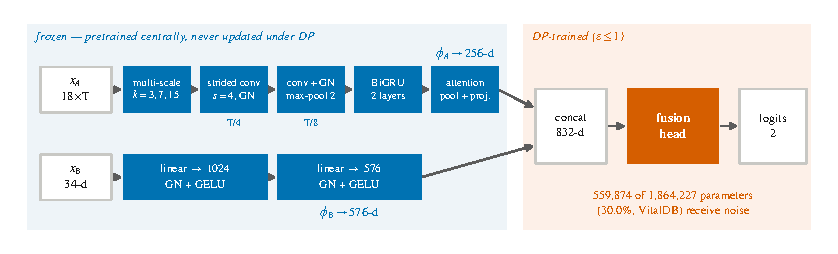
\includegraphics[width=\textwidth]{fig2_backbone.pdf}
\caption{Encoder--fusion backbone and the privacy boundary. Both encoders are
pretrained centrally and frozen; only the fusion head is trained under
differential privacy, so noise is applied to $559{,}874$ of $1{,}864{,}227$
parameters. Section~\ref{sec:method:backbone} defines the two pretraining
configurations, and Section~\ref{sec:exp:impl} records which produced which
result. No batch normalization appears anywhere, because it mixes statistics
across a batch and would make the per-patient gradient ill-defined.}
\label{fig:backbone}
\end{figure*}

Two properties of the backbone are required by the privacy mechanism. First,
its parameters remain frozen throughout federated training, so all trainable
and privatized capacity resides in the fusion head, which holds $559{,}874$ of
the $1{,}864{,}227$ parameters. The private optimization is therefore close to
a linear probe over fixed features. Second, every normalization layer is a
group or layer normalization; no batch normalization is used. Batch
normalization mixes statistics across the examples of a batch, so per-example,
and therefore per-patient, gradients would not be well defined, and the
privacy accounting would be invalid. The recurrent layer is likewise
implemented in a form compatible with per-sample gradients.

The pretraining corpus must satisfy an additional condition. If the encoders
are pretrained on data from the federated clients, they have been exposed to
the protected population without a guarantee, and the budget reported for the
head does not describe the system end to end. PP-HFM therefore distinguishes
two encoder configurations.

In the \emph{oracle} configuration, the encoders are pretrained on the pooled
training data of the federated clients. This configuration does \emph{not}
provide a valid end-to-end guarantee and is not proposed for deployment. It is
used to characterize the mechanism, because it isolates the attainable
performance of the head-only recipe from the origin of the representation. In
the \emph{disjoint} configuration, a set of individuals is reserved before
federated training, disjoint at the individual level from every client's
training, validation and test splits, and the encoders are pretrained only on
this set. Disjointness is verified explicitly. This configuration provides the
guarantee claimed in this paper, and its utility cost is measured.
Section~\ref{sec:exp:impl} specifies which configuration produced each result,
and Section~\ref{sec:results:objectives} reports the cost of moving between
them.

\subsection{Patient-Level Privacy Mechanism}
\label{sec:method:threat}
\label{sec:method:privacy}

A clinical system must provide a guarantee about individuals, whereas the
standard mechanism provides one about records. Differentially private
stochastic gradient descent bounds the influence of a training \emph{record}
by clipping its gradient to a fixed norm and adding noise to the aggregate
\cite{ref6}. When each record corresponds to a distinct person, the two
coincide. In a monitoring dataset, however, a record is a fixed-length window
and a single operation yields many windows, so removing one patient removes as
many records as that patient contributed. An $(\varepsilon,\delta)$-differentially
private mechanism is $(k\varepsilon,\,k e^{(k-1)\varepsilon}\delta)$-differentially
private for groups of size $k$ \cite{ref8}. Applied at the mean group size of
this cohort, this conversion turns a nominal $\varepsilon = 1$ into
$\varepsilon \approx 8$ with $\delta \approx 9 \times 10^{-2}$, which does not
support a clinical claim. The gap between the two units is illustrated in
Fig.~\ref{fig:sensitivity}.

Whether the two units differ depends on the deployment. When each client
corresponds to a single individual, as in a wearable installation where one
participant carries one device, client-level, user-level and individual-level
guarantees coincide. When a client holds records from many individuals, as an
institution holding many patients does, the units differ for every
participant. The mechanism below addresses the second case. The framework
applies to both, but only the second exhibits the gap, and the evaluation is
organized accordingly.

\begin{figure}[!t]
\centering
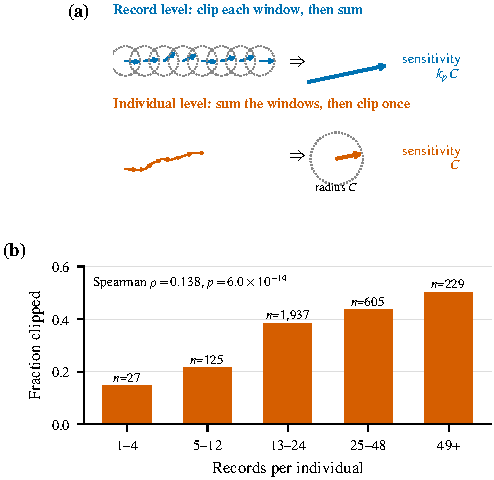
\includegraphics[width=\columnwidth]{fig02_privacy_unit.pdf}
\caption{Where the guarantee is decided. (a) Clipping each window to $C$ bounds
the influence of a \emph{window}: a patient contributing $k_p$ windows can
still displace the aggregate by $k_p C$. Summing a patient's windows before
clipping bounds the influence of the \emph{patient} at $C$, however many
windows that patient contributed. (b) On eICU at $C = 1$, the fraction of
individuals whose summed gradient is clipped rises with the number of records
they contribute; bar labels give individuals per bin.}
\label{fig:sensitivity}
\end{figure}

The mechanism enforces the guarantee at the point of clipping rather than by
conversion afterwards. The sampling unit is the patient: at each optimization
step, a client samples patients independently at a fixed rate, so the rate
entering the accountant is defined over patients rather than windows. For each
sampled patient, the gradients of all of that patient's windows are summed into
one per-patient gradient, and this sum is clipped to the clipping norm.
Clipping the sum makes the sensitivity patient-level: a patient can change the
aggregate by at most the clipping norm regardless of the number of windows,
whereas clipping each window separately would allow a change proportional to
that number. Gaussian noise calibrated to the same norm is then added once per
step to the aggregate of the clipped per-patient gradients, the result is
divided by the \emph{expected} batch size $q|\mathcal{P}_k|$, and the head
parameters are updated. The divisor must not be the realized batch size $|S|$:
the noise norm reveals the divisor, and $|S|$ depends on whether a given
patient is present, so normalizing by it releases information the accountant
does not cover. For the same reason a step whose sample is empty still
releases the noise. The mechanism is stated in
Algorithm~\ref{alg:patientdp}. For compute, at most $64$ records of a patient
enter its summed gradient; the rule is fixed and public, so the guarantee is
unaffected, and it truncates $4.1\,\%$ of eICU patients ($3.5\,\%$ of
training windows) and no VitalDB patient.

\paragraph{Objective solved} Without clipping, the expected step of client
$k$ is $|\mathcal{P}_k|^{-1}\sum_{p}g_p = \bar{k}_k\,\nabla F_k(\theta)$,
where $F_k$ is the record mean of the client's empirical risk and
$\bar{k}_k = n_k/|\mathcal{P}_k|$ the mean number of records per patient. A
local pass takes $|\mathcal{P}_k|/B$ such steps, $\bar{k}_k$ times fewer
than a record-level pass with $B$ records per step, so to first order in the
learning rate both displace client $k$ by $\eta\,(n_k/B)\,\nabla F_k$.
Before clipping, the patient-level mechanism therefore targets the declared
record-mean objective with unchanged client weights, in fewer and larger
steps. The argument is for the plain gradient step of
Algorithm~\ref{alg:patientdp}; the implementation passes the privatized
gradient to Adam, which is post-processing and leaves the guarantee unchanged
but rescales coordinates adaptively, so the argument holds only approximately.
Clipping is what changes the objective: each patient's summed gradient
is bounded as a whole, the surrogate of user-level DP-SGD \cite{ref11}, which
down-weights patients whose summed gradient exceeds $C$, typically those with
many records. This change belongs to the unit and is part of its measured
cost.

\begin{algorithm}[!t]
\caption{Patient-level private local update at client $k$}
\label{alg:patientdp}
\begin{algorithmic}[1]
\REQUIRE frozen $\theta_{\mathrm{enc}}$; head $\theta_{\mathrm{head}}$;
         patients $\mathcal{P}_k$ with records $\{W_p\}$; clip $C$;
         noise $\sigma$; rate $q$ from \eqref{eq:3}; step size $\eta$
\FOR{each local step}
  \STATE Sample $S \subseteq \mathcal{P}_k$, each $p$ independently w.p. $q$
  \FOR{$p \in S$}
    \STATE $g_p \leftarrow \sum_{(x,y)\in W_p}
            \nabla_{\theta_{\mathrm{head}}} \ell(f_\theta(x),y)$
            \hfill $\triangleright$ group by patient
    \STATE $\bar g_p \leftarrow g_p \cdot \min(1, C/\lVert g_p\rVert_2)$
            \hfill $\triangleright$ bound the sum
  \ENDFOR
  \STATE $\tilde g \leftarrow \frac{1}{q\,|\mathcal{P}_k|}\big(\sum_{p\in S}\bar g_p
          + \mathcal{N}(0,\sigma^2C^2I)\big)$
          \hfill $\triangleright$ also when $S=\emptyset$
  \STATE $\theta_{\mathrm{head}} \leftarrow \theta_{\mathrm{head}} - \eta\,\tilde g$
  \STATE Accountant.step($\sigma$, $q$)
\ENDFOR
\RETURN $\theta_{\mathrm{head}}$
\end{algorithmic}
\end{algorithm}

Accounting uses the same patient-level sampling rate, so the reported budget is
patient-level by construction. A single accountant instance persists for the
whole of a client's participation, so composition across rounds is preserved.
The construction has two costs, which this work measures: the number of
effective units per step decreases from windows to patients, and a patient with
many windows has their summed gradient clipped more strongly than a patient with
few. The dependence of this cost on the number of records per individual is
examined empirically by holding the first effect fixed and varying the second
(Section~\ref{sec:results:kscaling}).

\subsection{Noise Calibration Across Heterogeneous Clients}
\label{sec:method:calib}

The noise multiplier determines the budget for a given clipping norm, and
depends on the sampling rate and on the number of optimization steps of a
client. In a federated system partitioned by institution or specialty, these
quantities differ substantially between clients: a small client samples a
large fraction of its population per step, whereas a large client samples a
small one. A single noise multiplier calibrated for the most demanding client
satisfies the budget everywhere, but imposes that client's noise on every
other; on the external corpus, a hospital of fifteen patients sampled at rate
one sets the multiplier for all $187$ clients.

When each patient is held by exactly one client, as (A1) requires, the clients'
mechanisms act on disjoint sets of individuals, and by parallel composition the
guarantee for a patient is that of the client that holds them; individuals held
by several clients are treated where the scope of the theorem is stated. Each client therefore receives
its own noise multiplier $\sigma_k$, the smallest that meets the training
budget for that client's sampling rate and step count, Eq.~\eqref{eq:6}. The
multiplier depends only on the public client size, so it releases nothing
further. Accounting uses the privacy loss distribution accountant \cite{ref33},
which gives a tighter upper bound than R\'enyi accounting for the same
mechanism. The comparisons between arms in Section~\ref{sec:results:unit} use
the single most conservative multiplier, the maximum of $\sigma_k$, with
R\'enyi accounting, which holds every arm to the same noise.

Two details are essential. First, the number of optimization steps entering
the calibration must be the number the client actually executes; a count that
is too low underestimates the required noise. Second, the population and
sampling rate of each client are read from the partition files used in
training rather than from cached metadata, because metadata that no longer
matches the data produces a budget that is violated without any warning. Both
details are stated as part of the method because violations of either are not
detectable from training logs and can only be found by independent
recomputation.

\subsection{Two-Tier Hierarchical Aggregation}
\label{sec:method:agg}

In a flat federated system, every client update is sent to the cloud in every
round, so the wide-area link limits the update frequency. An intermediate
aggregation tier removes this limitation \cite{ref2, ref3}: several rounds of
local optimization and edge averaging are performed for each round of cloud
averaging, so the wide-area link is used once per group of local rounds.
PP-HFM adopts this organization, with $\tau_e$ edge rounds per cloud round, and
claims no novelty for the averaging rule.

Aggregation is performed in two stages, each weighted by the fixed number
of training records of the participants. The weights are public constants: a
weight computed from the records drawn in a given round would depend on which
patients were sampled and would reach the edge unprotected. Within a cloud round, each client
initializes from its edge model, performs one private local pass, and sends its
encoded update. The edge computes the weighted average over its clients and
returns it, and this is repeated $\tau_e$ times. The edges then report to the
cloud, which computes the weighted average over edges and broadcasts it as the
global model for the next round. Non-floating-point parameters are passed
through unchanged. The procedure is given in Algorithm~\ref{alg:round}.

\begin{algorithm}[!t]
\caption{PP-HFM cloud round $r$}
\label{alg:round}
\begin{algorithmic}[1]
\REQUIRE global model $\theta^{(r-1)}$; edge map $e(\cdot)$; edge rounds $\tau_e$
\STATE $\theta_e^{(r,0)} \leftarrow \theta^{(r-1)}$ for all edges $e$
\FOR{$s = 1$ \TO $\tau_e$}
  \FOR{each client $k$ \textbf{in parallel}}
    \STATE $\theta_k^{(r,s)} \leftarrow$ Algorithm~\ref{alg:patientdp}
           from $\theta_{e(k)}^{(r,s-1)}$
    \STATE Transmit $Q\big(\text{top-}\kappa(\theta_k^{(r,s)}-\theta_{e(k)}^{(r,s-1)})\big)$
  \ENDFOR
  \STATE Each edge aggregates by \eqref{eq:8}
\ENDFOR
\STATE Cloud aggregates by \eqref{eq:9} and broadcasts $\theta^{(r)}$
\RETURN $\theta^{(r)}$
\end{algorithmic}
\end{algorithm}

The parameter $\tau_e$ controls the trade-off of the hierarchy. With
$\tau_e = 1$, the edge tier is merged into the cloud tier, which recovers
conventional single-tier federated averaging; this configuration is used to
isolate the contribution of the hierarchy. Larger values reduce wide-area
transmissions proportionally but allow edge models to diverge further between
synchronizations. Because the privacy mechanism operates entirely within a
client and aggregation uses only privatized updates, $\tau_e$ affects
communication and convergence, and enters the guarantee only through the
number of optimization steps, which the calibration already accounts for.

\subsection{Update Encoding}
\label{sec:method:encoding}

A further component is adopted from established practice and is not claimed
as a contribution. It reduces the transmitted payload. Each
client update is sparsified by retaining only its largest-magnitude
coordinates, and the retained values are uniformly quantized to a reduced bit
width. The residual removed by sparsification is stored locally and added to
the next round's update, so suppressed coordinates are transmitted later rather
than lost. The encoding is applied after the privacy mechanism and is therefore
post-processing; by the post-processing property of differential privacy, it
does not affect the guarantee and can be tuned for bandwidth alone.

A private conformal threshold, released per client by the exponential
mechanism over ranks \cite{ref30, ref24} at $\varepsilon_{\mathrm{conf}} = 0.1$
with one score per calibration patient, was also evaluated. At about a hundred
calibration patients per client it does not attain coverage
(Section~\ref{sec:results}), so it is not part of the system, and the reported
budget is the training budget alone.

\subsection{Deployment Path and Inference Under a Latency Budget}
\label{sec:method:deploy}

The clinical value of the trained model depends on the delay between the
availability of a measurement and the return of a prediction, which is a
property of the deployment path. This path is therefore specified as part of
the system. The trained network is exported to a portable computation graph and executed
at full precision. Post-training eight-bit quantization \cite{ref26} was
evaluated as an alternative and rejected, because on a CPU provider it
increased rather than reduced latency (Section~\ref{sec:results}). Any
transformation of the released model after federated training is
post-processing and does not affect the privacy guarantee. Inference is executed at the edge tier rather
than in the cloud, so the wide-area link is not on the critical path.

The delay is decomposed into four separately measured stages, because an
end-to-end figure within budget may still be dominated by a removable stage.
Preprocessing constructs and normalizes the input tensors from the sensor
stream; the forward pass evaluates the exported graph; the threshold step of the evaluated conformal set, which is not deployed, is
kept as a conservative upper bound; and
a final stage converts the output into the format required by the consuming
system.

Latency is characterized by its distribution rather than its mean, and the
budget must be met at the 95th percentile, since a clinical service level is
defined by its tail. The measurement configuration is fixed in advance: the
full-precision graph is executed on a general-purpose CPU provider,
representing an edge node without an accelerator, for one thousand timed runs
after one hundred discarded warm-up runs, and each of the four stages is timed
within every run. A CPU provider is used because an edge deployment cannot be
assumed to have a GPU.

\subsection{Network and Energy Instrumentation}
\label{sec:method:instr}

Three of the four design objectives concern quantities that cannot be observed
from training: the wide-area traffic of the hierarchy, the reliability of update
delivery, and the energy consumed per round by each tier. These are properties
of the deployed topology and are therefore measured on simulated models of that
topology rather than estimated from parameter counts.

The network is modeled with the three tiers of Section~\ref{sec:method:arch}.
The device-to-edge segment uses a wireless local-area link and the
edge-to-cloud segment a point-to-point backhaul, so the asymmetry between
frequent local exchange over a low-cost link and infrequent global exchange
over a high-cost link is represented explicitly. Each round is simulated in
both directions, the downlink broadcast of the global model and the uplink
transmission of client updates. Traffic volume, delivery reliability and
end-to-end delay are recorded per round for the proposed configuration and for
the flat and centralized baselines. Per-round delay quantifies the latency
benefit of the hierarchy during training, which is distinct from the inference
latency of the deployment path in Section~\ref{sec:method:deploy}. Because the
payload is the compressed update of Eqs.~\eqref{eq:10}--\eqref{eq:11}, the
measured traffic is that of the specified system rather than of an
uncompressed approximation.

Energy is modeled per tier from the power characteristics of the hardware and
the completion time of the assigned work. The device tier represents
constrained embedded nodes, the edge tier server-class accelerated hardware,
and the cloud tier the aggregation host. Energy is reported per tier because a
hierarchical design redistributes work rather than reducing it, and an
aggregate figure would not show whether a saving at one tier is offset by an
increase at another.

The targets for these quantities were fixed in advance and are listed in
Table~\ref{tab:objectives}. The measured values are reported in
Section~\ref{sec:results}.

\begin{table}[!t]
\centering
\caption{Design objectives and their pre-registered targets. The problem
specification fixes a numeric threshold for communication reduction but asks
only that the latency benefit of the hierarchy be quantified, so O1b is stated
as a direction rather than a percentage. Measured values are reported in
Section~\ref{sec:results}.}
\label{tab:objectives}
\begin{tabular}{llc}
\toprule
& Quantity & Target \\
\midrule
O1  & Uplink traffic reduction vs.\ centralized & $\ge 50\%$ \\
O1b & Training-round latency vs.\ centralized   & improvement \\
O2a & Privacy budget, composed total            & $\varepsilon \le 1$ \\
O2b & Accuracy loss under the budget            & $\le 2$ pp \\
O3a & Inference latency, 95th percentile        & $< 100$ ms \\
O3b & Successful model updates                  & $> 99\%$ \\
O4  & Energy saving per round vs.\ centralized  & $\ge 20\%$ \\
\bottomrule
\end{tabular}
\end{table}

\subsection{Empirical Auditing of the Guarantee}
\label{sec:method:mia}

A differential privacy guarantee is an upper bound on the influence of an
individual. It does not show what an adversary achieves in practice, nor that a
system with a weaker guarantee is exploitable. Membership inference provides
this complementary measurement \cite{ref14}. PP-HFM is audited by
individual-level membership inference. Members are the patients in the
clients' training splits and non-members are patients held out entirely. Both
groups are scored by the same released model using the same procedure, so any
separation between them reflects membership.

Two attacks of different strength are used. The first compares each patient's
mean per-record loss with a global threshold \cite{ref15}. Aggregation to the
patient level before thresholding is essential: a per-record attack measures
record membership, which a record-level guarantee already protects, whereas
averaging over a patient's records converts weak per-record signals into a
per-individual signal. The second is a likelihood-ratio attack \cite{ref17}
adapted so that the unit of membership is the patient. Shadow models are
trained on independently sampled halves of the patient population, with all
records of a patient assigned together, and each shadow is trained with the
same recipe as the target model. For each patient, the distribution of a
logit-scaled confidence statistic is estimated separately over the shadows that
include and exclude that patient, and membership is scored by the ratio of the
two densities. A global threshold is confounded by per-patient difficulty, so
the attack strength it reports is a lower bound on leakage rather than an
estimate \cite{ref16}. Per-patient calibration removes this confound, as
illustrated in Fig.~\ref{fig:lira}.

\begin{figure}[!t]
\centering
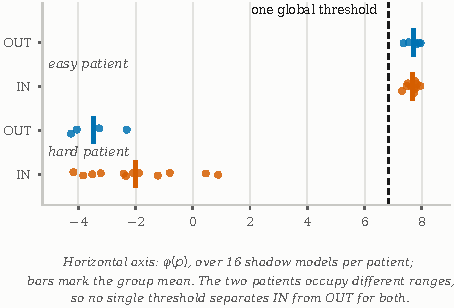
\includegraphics[width=\columnwidth]{fig4_lira.pdf}
\caption{Why per-patient calibration is necessary. Under a single global
threshold an easy non-member can outscore a hard member, so membership signal
is buried in per-patient difficulty. Fitting each patient's own in- and
out-distributions from shadow models removes that confound and scores
membership as a likelihood ratio.}
\label{fig:lira}
\end{figure}

Attacks are evaluated by the area under the receiver operating characteristic
curve and by the true-positive rate at low false-positive rates, because an
attack close to chance on average may still identify a few individuals with
high confidence. When the number of non-members is too small to resolve a
given false-positive rate, the value is reported as undefined rather than
interpolated.

A negative audit result is informative only if the attack is capable of
detecting leakage. The same procedure is therefore applied to a configuration
known to memorize, namely non-private training of the same head over the same
frozen encoders, and is required to detect clearly elevated leakage there. This
positive control is a precondition of the audit and is reported with every
result it qualifies.

% FLOAT NOTE: both algorithm floats are declared beside the text that cites
% them, not at the end of the section. Declared at the end — after the
% equations — LaTeX had no Methodology page top left and pushed Algorithm 2
% forward into Experimental Setup. A float never moves backwards; it must be
% declared where it can still be placed.
\subsection{Training Objective and Privacy Accounting}
\label{sec:method:objective}

Let $K$ clients be indexed by $k$, with client $k$ holding a local dataset
$\mathcal{D}_k$ of $n_k$ records and $n = \sum_k n_k$. Clients are assigned to
edges by a fixed map $e(\cdot)$. The records of client $k$ are partitioned by
individual into a set of patients $\mathcal{P}_k$, and $W_p$ denotes the
records contributed by patient $p$, with $k_p = |W_p|$; the partition is
constructed so that $W_p$ never spans two clients or two evaluation splits,
which holds by construction on eICU and on the person-level VitalDB partition
(Section~\ref{sec:experiments}).
Model parameters are written $\theta = (\theta_{\mathrm{enc}},
\theta_{\mathrm{head}})$, and $\ell$ is the cross-entropy; the loss is unweighted, because class
weights computed from the training labels would be a further unprotected
release. The
notation is summarized in Table~\ref{tab:notation}.

\begin{table}[!t]
\centering
\caption{Notation.}
\label{tab:notation}
\begin{tabular}{ll}
\toprule
Symbol & Meaning \\
\midrule
$K$, $E$              & number of clients, of edge aggregators \\
$\mathcal{P}_k$, $W_p$ & patients at client $k$; records of patient $p$ \\
$k_p = |W_p|$         & records contributed by patient $p$ \\
$R$, $\tau_e$         & cloud rounds; edge rounds per cloud round \\
$B$                   & patients sampled per optimization step \\
$C$, $\sigma$         & clipping norm; noise multiplier \\
$q$                   & Poisson sampling rate over patients \\
$(\varepsilon,\delta)$ & privacy budget \\
$\theta_{\mathrm{enc}}$, $\theta_{\mathrm{head}}$ & encoder, fusion-head parameters \\
\bottomrule
\end{tabular}
\end{table}

The learning objective is the standard weighted empirical risk over clients,
\begin{equation}
\begin{aligned}
\min_{\theta}\; F(\theta) &= \sum_{k=1}^{K} \frac{n_k}{n} F_k(\theta), \\
F_k(\theta) &= \frac{1}{n_k}\!\!\sum_{(x,y)\in\mathcal{D}_k}\!\!
               \ell\big(f_\theta(x), y\big),
\end{aligned}
\tag{1}
\label{eq:1}
\end{equation}
minimized only over $\theta_{\mathrm{head}}$, since $\theta_{\mathrm{enc}}$ is
pretrained on a disjoint public population and held fixed,
\begin{equation}
\theta_{\mathrm{enc}}\ \text{fixed},
\qquad
\theta_{\mathrm{head}} \leftarrow \text{privately optimized}.
\tag{2}
\label{eq:2}
\end{equation}

At each optimization step client $k$ draws a subset $S \subseteq \mathcal{P}_k$
by including each patient independently with probability
\begin{equation}
q_k = \min\!\Big(1,\ \frac{B}{|\mathcal{P}_k|}\Big),
\tag{3}
\label{eq:3}
\end{equation}
a rate defined over patients rather than records, which makes the accounted
quantity patient-level. For each sampled
patient the record gradients are accumulated and the sum is bounded,
\begin{equation}
\begin{aligned}
g_p &= \!\!\sum_{(x,y)\in W_p}\!\! \nabla_{\theta_{\mathrm{head}}}\,
       \ell\big(f_\theta(x), y\big), \\
\bar{g}_p &= g_p \cdot \min\!\left(1, \frac{C}{\lVert g_p \rVert_2}\right).
\end{aligned}
\tag{4}
\label{eq:4}
\end{equation}
Equation~\eqref{eq:4} determines the unit of the guarantee: because the bound
is applied to the sum, the influence of patient
$p$ is at most $C$ irrespective of $k_p$, whereas bounding each record
separately would admit an influence of $k_p C$. A single perturbation scaled to
the same norm is then applied to the aggregate,
\begin{equation}
\tilde{g} = \frac{1}{q_k |\mathcal{P}_k|}\left( \sum_{p \in S} \bar{g}_p
+ \mathcal{N}\!\big(0, \sigma^2 C^2 I\big) \right),
\tag{5}
\label{eq:5}
\end{equation}
where the divisor is a public constant rather than the realized $|S|$,
and the head is updated by $\theta_{\mathrm{head}} \leftarrow
\theta_{\mathrm{head}} - \eta\,\tilde{g}$.

Each client uses the smallest noise multiplier that meets the training budget
for its own sampling rate and step count,
\begin{equation}
\sigma_k = \min\big\{\sigma :\;
\varepsilon_k\big(\sigma,\, q_k,\, T_k\big)
\le \varepsilon\big\},
\tag{6}
\label{eq:6}
\end{equation}
where $\varepsilon_k$ is obtained from the privacy loss distribution accountant
\cite{ref33}, or from a R\'enyi accountant \cite{ref7, ref29} for the
single-multiplier arms $\sigma^{\star} = \max_k \sigma_k$, and the step count
is the number the client executes,
\begin{equation}
T_k = R\,\tau_e\,\max\!\Big(1, \Big\lfloor \frac{|\mathcal{P}_k|}{B} \Big\rfloor\Big)
\tag{7}
\label{eq:7}
\end{equation}
for the patient sampler of Algorithm~\ref{alg:patientdp}. $T_k$ must equal
the executed count; a count that differs from the executed one yields a budget
that is violated without any observable symptom.

Aggregation applies the weighted average at each tier. Writing
$\theta_k^{(r,s)}$ for the model of client $k$ after edge round $s$ of cloud
round $r$,
\begin{equation}
\theta_e^{(r,s)} = \!\!\sum_{k :\, e(k)=e}\!\!
\frac{n_k}{\sum_{j : e(j)=e} n_j}\; \theta_k^{(r,s)},
\tag{8}
\label{eq:8}
\end{equation}
\begin{equation}
\theta^{(r)} = \sum_{e=1}^{E} \frac{N_e}{\sum_{e'} N_{e'}}\;
\theta_e^{(r,\tau_e)},
\qquad
N_e = \!\!\sum_{k : e(k)=e}\!\! n_k .
\tag{9}
\label{eq:9}
\end{equation}

Updates are encoded before transmission. Sparsification retains the
$\kappa d$ largest-magnitude coordinates of an update $\Delta$ of dimension
$d$,
\begin{equation}
[\Delta^{\mathrm{sp}}]_i =
\begin{cases}
[\Delta]_i, & i \in \operatorname*{arg\,top}_{\kappa d} |\Delta| \\
0, & \text{otherwise,}
\end{cases}
\tag{10}
\label{eq:10}
\end{equation}
and the retained values are quantized uniformly to $b$ bits with step
$s = (v_{\max}-v_{\min})/(2^{b}-1)$,
\begin{equation}
Q(v) = v_{\min} + \operatorname{round}\!\Big(\frac{v - v_{\min}}{s}\Big)\, s .
\tag{11}
\label{eq:11}
\end{equation}
The residual $\Delta - \Delta^{\mathrm{sp}}$ is accumulated locally and added
to the next round's update. Both operations act on the already-perturbed
quantity of Eq.~\eqref{eq:5} and are therefore post-processing.


The guarantee is stated formally below. Two datasets are \emph{neighboring} if
one is obtained from the other by adding or removing every record of a single
patient. Three conditions are assumed. (A1) Each patient's records lie in the
training split of exactly one client, and the training, validation and test
cohorts are disjoint in patients. (A2) The following are public: the
architecture, the encoder parameters $\theta_{\mathrm{enc}}$, which are
pretrained on a patient-disjoint public pool, all hyperparameters
$(R,\tau_e,B,C,\sigma,\eta,\kappa,b)$, the edge map, the input standardization constants, and the declared client
sizes $|\mathcal{P}_k|$ and $n_k$, which are fixed before training; $q_k$,
$T_k$, $\sigma_k$ and the aggregation weights are computed from them and never
from the data.
(A3) The forward pass of a record depends on that record alone; the model
contains no normalization across records, such as batch normalization, so the
gradient of one patient's records is unaffected by any other patient.

\begin{theorem}[Patient-level guarantee]
\label{thm:guarantee}
Under (A1)--(A3), let each $\sigma_k$ satisfy Eq.~\eqref{eq:6}. The transcript of a
PP-HFM run, consisting of every encoded client update, every edge and cloud
model, and the model selected on the validation cohort, is
$(\varepsilon,\delta)$-differentially private with respect to
each training patient, under adding or removing all records of one patient
with the parameters of (A2) held fixed.
\end{theorem}

\begin{IEEEproof}
Fix a training patient $p$, held by client $k$ by (A1). \emph{One step.} Given
the model entering a step, the per-patient gradients $\bar g_{p'}$,
$p' \neq p$, are unchanged by the presence of $p$ by (A3), and
$\lVert \bar g_p \rVert_2 \le C$ by Eq.~\eqref{eq:4}. The noisy sum in
Eq.~\eqref{eq:5} is therefore a Poisson-subsampled Gaussian mechanism with rate
$q_k$, noise $\sigma C$ and $\ell_2$-sensitivity $C$ under addition or removal
of $p$, whose privacy loss is bounded in \cite{ref29, ref33}. Division by the
public constant $q_k|\mathcal{P}_k|$ and the optimizer update are
post-processing. \emph{Composition at client $k$.} Each step takes as input the
outputs of earlier steps, of other clients and public quantities, so the $T_k$
steps compose adaptively, and R\'enyi divergences add \cite{ref7}. The
accountant evaluates the composed bound exactly for $(\sigma,q_k,T_k)$, and
Eq.~\eqref{eq:6} ensures $\varepsilon_k \le \varepsilon$ at
$\delta$. Because $\sigma_k$ is a function of the public $|\mathcal{P}_k|$ and
$T_k$ only, using a different multiplier at each client releases nothing. \emph{Other clients.} By (A1) no other client accesses
the records of $p$; its outputs are randomized functions of its own data,
public quantities and messages already released, and therefore contribute no
privacy loss with respect to $p$. \emph{The hierarchy.} Sparsification with a
locally stored residual, quantization, edge and cloud averaging with the public
weights of Eqs.~\eqref{eq:8}--\eqref{eq:9}, and broadcast are functions of
released outputs and public quantities, and selection on the validation cohort
uses data disjoint from $p$ by (A1); all are post-processing.
\end{IEEEproof}

\begin{corollary}[Coincidence of the units]
\label{cor:k1}
If every patient contributes one record, Algorithm~\ref{alg:patientdp} is
differentially private stochastic gradient descent with Poisson sampling over
records at rate $q_k$, with the same clipping norm and noise. For equal
$(B, T_k, \sigma, C)$ the patient-level and record-level mechanisms are the
same mechanism, so a difference between them at one record per patient
measures seed variation or an implementation difference, not a property of the
privacy unit.
\end{corollary}

The theorem bounds what the guarantee reveals; the next statement predicts what
it costs. In the scaling experiments of Section~\ref{sec:results:kscaling},
$P$ individuals each contribute exactly $k$ records, so the record-level arm
minimizes $F(\theta) = \frac{1}{Pk}\sum_{p}\sum_{w \in W_p} \ell_w(\theta)$
and the individual-level arm minimizes the same $F$ written as
$\frac{1}{P}\sum_p \bar\ell_p(\theta)$, with
$\bar\ell_p = \frac{1}{k}\sum_{w\in W_p}\ell_w$.

\begin{proposition}[Cost in records per individual]
\label{prop:scaling}
Let each $\ell_w$ be convex and $L$-Lipschitz on a parameter domain of diameter
$D$ in $\mathbb{R}^d$, and let both arms be trained by differentially private
gradient descent at the same $(\varepsilon,\delta)$, and let
$\Lambda = LD\sqrt{d\log(1/\delta)}/\varepsilon$.
(i) The excess empirical risk of the record-level arm is at most
$c_{\mathrm{rec}}\Lambda/(Pk)$ and that of the individual-level arm at most
$c_{\mathrm{ind}}\Lambda/P$, with constants independent of $k$; both rates are
tight in the worst case up to logarithmic factors. (ii) If both arms attain their rate with a common
constant $c$, the gap is $A(1 - 1/k)$ with $A = c\Lambda/P$.
\end{proposition}

\begin{IEEEproof}
For $n$ units with convex $L$-Lipschitz losses, private gradient descent attains
excess empirical risk $O(LD\sqrt{d\log(1/\delta)}/(n\varepsilon))$, and this rate
is tight up to logarithmic factors \cite{ref31}. The record-level arm has $n = Pk$ units. In the
individual-level arm the unit is $\bar\ell_p$, which is $L$-Lipschitz as an
average of $L$-Lipschitz losses; clipping the summed gradient at $C$ equals
clipping the gradient of $\bar\ell_p$ at $C/k$, a rescaling that leaves the
guarantee unchanged, so the mechanism is private gradient descent over $n = P$
units. This gives (i), and (ii) follows by subtraction.
\end{IEEEproof}

Part (ii) rests on an assumption that (i) does not supply: upper bounds with
different constants do not determine the attained gap. The form $A(1-1/k)$ is
therefore a \emph{scaling hypothesis} that the proposition motivates, not a
theorem, and it is tested empirically, including out of sample. Moreover, the
proposition concerns bounds for convex losses, whereas the head is not convex
and the reported metric is average precision rather than excess risk. The
hypothesis therefore concerns the \emph{shape} of the cost, not its magnitude:
a gap of the form $A(1 - 1/k)$ with one free parameter, zero at $k = 1$, and an
individual-level arm whose utility does not depend on $k$. It also identifies
what would recover the cost. Additional records per individual reduce the
variance of $\bar\ell_p$'s gradient, but a clipping bound fixed around zero
cannot exploit this; mechanisms that clip around an estimate of the
per-individual mean can, and attain user-level rates that improve with $k$
\cite{ref32}. Rescaling the summed gradient by the record count, tested in
Section~\ref{sec:results:kscaling:nd}, is not such a mechanism.

The theorem fixes what is and is not covered. On eICU and on the
person-level VitalDB partition the unit is the person. On the case-level
VitalDB partition the unit is the surgical case: $230$ of $5{,}974$ people
($3.9\,\%$) underwent more than one operation, and for them the guarantee
holds per operation and extends to the person only by group privacy over at
most $14$ cases, composed across clients for the $68$ training persons whose
cases lie on two. On eICU, where clients are hospitals, the stays of $2{,}177$ of $74{,}327$ training persons ($2.9\,\%$) lie at two to four hospitals, so in the source partition (A1) fails for them. The privacy-cost and end-to-end runs therefore use a partition in which each such person is moved, with all their records, to the hospital holding most of their stays ($49{,}939$ training records; likewise $509$ validation and $589$ test persons); no record is excluded and every split is unchanged. In that partition every training and validation person is held by one hospital, so (A1) holds and the guarantee is $\varepsilon_{\mathrm{train}} = 0.9$ for every training person, verified independently for every client of every run (privacy-loss-distribution bounds $[0.880, 0.900]$; R\'enyi accountant $0.974$), and the evaluated conformal release adds $\varepsilon_{\mathrm{conf}} = 0.1$ once per person. The remaining eICU analyses (system objectives other than O2, scaling grid, clipping rule and prior systems) use the source partition, in which the per-client budget composes across the hospitals that hold a person: with the headline accountant, at most $1.32$, $1.64$ and $1.92$ for the $2{,}097$, $75$ and $5$ persons at two, three and four hospitals (R\'enyi: $1.42$, $1.77$, $2.08$), and at most $m\varepsilon$ in general; arms compared with each other share the partition. On the wearable deployment each client is one participant, and the
mechanism evaluated there is record-level; a person-level guarantee would
require client-level privacy at the edge, which is not evaluated. Outside the
guarantee are the validation cohort, which is used without noise for checkpoint
selection, the input standardization constants, which are computed once from
the training cohort, and the declared client sizes, which are treated as
public, as is conventional for privately trained models \cite{ref6}. Adding or
removing a patient changes the realized cohort but not the mechanism, because
every parameter is fixed by the declared sizes before training; this is the
setting in which the Poisson-subsampled Gaussian is analyzed
\cite{ref29, ref33}. In the experiments the declared sizes equal the realized
cohort sizes; where a size is sensitive, it can be replaced by a coarse public
value or released by a private count, and the theorem holds for whichever
declared values are used. Table~\ref{tab:scope} lists, for each evaluated configuration, the unit,
the provenance of the encoders and standardization constants, the accounting
and what the guarantee covers. The implementation of the accounting is
additionally checked by a suite of 17 regression checks, seven of which cover
it: composition of the budget across calls, release and accounting of noise at
every step with the expected-batch divisor, one conformal score per calibration
patient, and per-client multipliers within the budget. These are
implementation-level checks of the accounting configuration; they do not by
themselves establish the guarantee.

\begin{table*}[!t]
\centering
\caption{Scope of the guarantee in each evaluated configuration}
\label{tab:scope}
\footnotesize
\setlength{\tabcolsep}{4pt}
\begin{tabular}{>{\raggedright\arraybackslash}p{4.8cm}>{\raggedright\arraybackslash}p{2.3cm}>{\raggedright\arraybackslash}p{3.6cm}>{\raggedright\arraybackslash}p{3.3cm}>{\raggedright\arraybackslash}p{2.7cm}}
\toprule
Configuration & Unit & Encoders / standardization & Accounting & Guarantee covers \\
\midrule
eICU, headline (one hospital per person) & patient & disjoint / training cohort & $\sigma_k$, PLD; $0.9 + 0.1$ & training transcript \\
eICU, pool-fitted constants (one hospital per person) & patient & disjoint / public pool & $\sigma_k$, PLD; $0.9 + 0.1$ & end to end \\
VitalDB, person-level headline & person & oracle / training cohort & $\sigma_k$, PLD; $0.9 + 0.1$ & transcript; (A2) violated \\
VitalDB, disjoint encoders (case-level) & surgical case & disjoint / training cohort & $\sigma_k$, PLD; $0.9 + 0.1$ & transcript, per case \\
VitalDB, cost of the unit and audit (person-level) & person vs record & oracle / training cohort & $\sigma_{\max}$, RDP; $1.0 + 0.5$ & training transcript \\
Scaling grids, clipping rule (VitalDB case-level; eICU) & individual vs record & oracle (VitalDB), disjoint (eICU) / training & $\sigma_{\max}$, RDP; $0.8$--$1.0 + 0.2$--$0.5$ & training transcript$^{\ddagger}$ \\
eICU, prior systems (source partition) & patient & disjoint / training cohort & $\sigma_k$, PLD; $0.9 + 0.1$ & training transcript$^{\ddagger}$ \\
WEAR & record (= participant) & oracle / training cohort & record-level; $0.766 + 0.2$ & transcript, per record \\
\bottomrule
\end{tabular}
\par\vspace{3pt}\parbox{\linewidth}{\footnotesize Unit: neighboring datasets differ by all records of one patient, person or case, or by one record; ``vs'' marks a comparison of two arms. Accounting: $\varepsilon_{\mathrm{train}} + \varepsilon_{\mathrm{conf}}$ at $\delta = 10^{-5}$; $\sigma_k$, per-client multipliers; $\sigma_{\max}$, one worst-client multiplier; PLD, privacy-loss-distribution accountant; RDP, R\'enyi accountant. The conformal release was evaluated and is not part of the deployed system. Arms compared with each other share one configuration. Other analyses (recipe, ablation, fusion, attribution) are labeled with their partition and mechanism in Section~\ref{sec:results}. $^{\ddagger}$eICU on the source partition: for the $97.1\,\%$ of training persons at one hospital; the $2.9\,\%$ at two to four hospitals compose the mechanisms of those hospitals ($\varepsilon_{\mathrm{train}} \le 1.32$--$1.92$ with $\sigma_k$ and PLD).}
\end{table*}

Finally, the audit statistic of Section~\ref{sec:method:mia} is the
logit-scaled confidence of a patient, averaged over that patient's records,
\begin{equation}
\varphi(p) = \frac{1}{|W_p|}\sum_{(x,y)\in W_p}
\Big( z_y(x) - \log\!\!\sum_{j \neq y} e^{z_j(x)} \Big),
\tag{12}
\label{eq:14}
\end{equation}
which is the numerically stable form of $\log\!\big(\hat{p}_y/(1-\hat{p}_y)\big)$,
and membership is scored by the ratio of the fitted in- and out-densities,
\begin{equation}
\Lambda(p) = \log
\frac{\mathcal{N}\!\big(\varphi(p);\, \mu_{\mathrm{in}}(p), \sigma^2_{\mathrm{in}}(p)\big)}
     {\mathcal{N}\!\big(\varphi(p);\, \mu_{\mathrm{out}}(p), \sigma^2_{\mathrm{out}}(p)\big)} .
\tag{13}
\label{eq:15}
\end{equation}



The objective in Eq.~\eqref{eq:1} is minimized over the fusion head only,
using the mechanism of Eqs.~\eqref{eq:3}--\eqref{eq:5} with the noise scale
given by Eq.~\eqref{eq:6}, while the encoders remain frozen. Optimization uses
stochastic gradient descent on the perturbed gradient. The reported model is
selected by validation performance.
